\section{Funktionsumfang der Beispiel Anwendung}
Grundsätzlich wurde beim Entwurf des Funktionsumfang versucht, die typischen Funktionalitäten von Applikationen abzubilden. Eine Befragung mobiler Anwendungsentwickler durch JetBrains ergab, dass die wichtigsten Funktionen Datenspeicherung, Kommunikation über Netzwerk, Medienanzeige, Status und Navigationsmanagment, Datensynchronisierung, Dateien lesen/schreiben, Sicherheit, Bezahlung, Berechnungen und Machine Learning sind\cite{JetBrains_miscellaneous_2021}. Natürlich sind gerade Machine Learning oder die Bezahlung eine sehr Anwendungsfallspezifische Sache, jedoch gibt diese Liste einen guten Eindruck, was eine typische App an Funktionalität benötigt.
Um den Arbeitsaufwand realistisch zu halten und trotzdem aber einige der oben genannten Parameter abzudecken, ist die Implementierung wie im Folgenden beschrieben eingeschränkt.

Allgemein soll eine App gebaut werden, die sich an einer bestehende Webanwendung orientiert und einen Teil der Funktionalität durch die Programmierung abbilden soll. Des weiteren wird eine GraphQL-Schnittstelle genutzt um die Daten der Webanwendung zu nutzen. 

\subsection{Nativer und Cross-kompilierter Ansatz}
Bei der Nativen und der Cross-kompilierten Applikation wird der in Abbildung \ref{fig:pageflow} dargestellten Ablauf abgebildet. Dabei sind diese komplett durch in der Applikation implementierten Seiten dargestellt. Diese sind eine Start-, Login- , Profil- , Kommunikations- und eine Chatseite. Dadurch werden die oben genannte Aspekte bis auf Bezahlung und Machine Learningaben abgedeckt. Denn durch den Login etwa erfüllt die Applikation teilweise die Bereiche Sicherheit, Statusmanagment, Daten lesen/schreiben und Kommunikation über Netzwerk. 

\begin{figure}[ht]
  \centering
  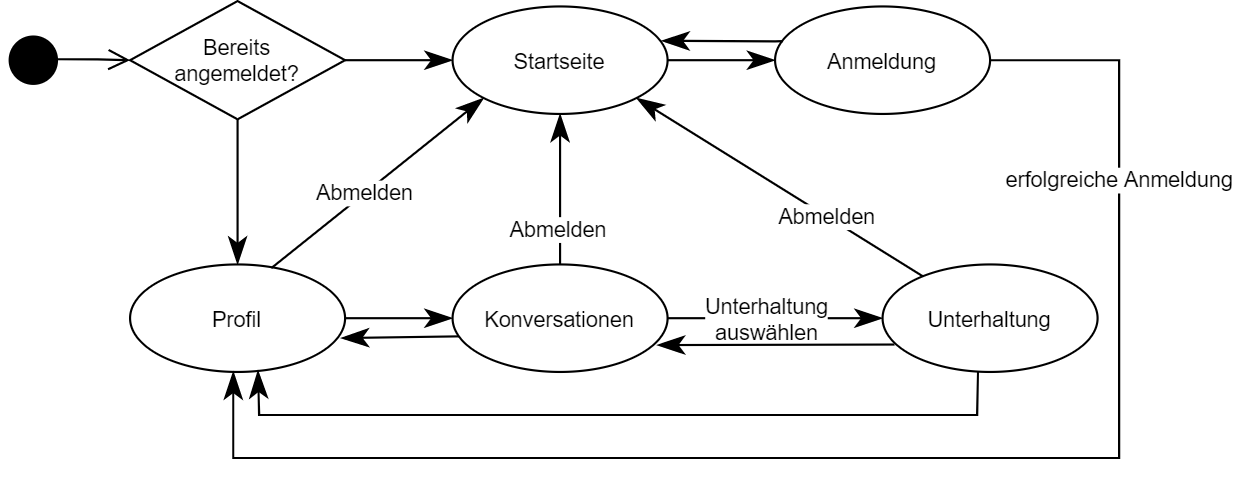
\includegraphics[height=7cm,keepaspectratio]{images/Pageflow_native_flutter.png} 
  \caption[Seitenablauf der implemierten nativen und Cross-kompilierten Applikation]{Verbindungen zwischen den Seiten der implementierten Applikation des nativen und des Cross-kompilierten Ansatzes}
  \label{fig:pageflow}
\end{figure}

Der genaue Ablauf der App ist dabei, dass der Nutzer die App öffnet. Wenn er bereits eingeloggt ist, wird er automatisch auf die Profil Seite übergeleitet, auf der eine über die Schnittstelle von einem Server abgefragte Liste angezeigt wird. Ist er jedoch nicht angemeldet, so landet er auf einer Startseite/ Willkommensseite. Über ein Menü erreicht der Nutzer die Loginseite, von der er nach erfolgreicher Anmeldung zu der bereits erwähnten Profilseite kommt. Über einen Knopf in der Menüleiste der App kann der eingeloggte Nutzer auf die Konversationsseite wechseln. Hier wird im eine Liste an Konversationen angezeigt, an denen er beteiligt ist. Durch die Auswahl einer Konversation gelangt er auf eine Unterhaltungsseite, auf der er die bereits bestehenden Nachrichten lesen und neue Nachrichten abschicken kann. Während der Nutzer angemeldet ist, kann er sich außerdem abmelden und damit wieder auf die Startseite weitergeleitet werden. Dabei werden die Zugangs- und andere Personendaten gelöscht.

\subsection{Hybrider und gemischter Ansatz}
Bei dem hybriden Ansatz wird lediglich die bereits bestehende Website in eine native programmierte Applikation eingebunden. Sie stellt dabei die Aufgabe nach, die bei diesem Ansatz eigentlich ein eigenes Framework übernehmen würde. Sie ist jedoch durch die spezifische Implementierung der Webseite stark in der Funktionalität eingeschränkt. Beim letzten Ansatz, dem gemischten Ansatz geht dies deutlich weiter. Hier wird zwischen der Webseite und mit einem Cross-kompilierten Framework erstellten Seiten hin und her geschaltet. Dabei wird insbesondere der Login die Profilseite und das Chat System ersetzt, während der Rest der Applikation aus der Webseite besteht. Außerdem wird in dieser Implementierung die Navigation der Webseite durch eine neu programmierte Navigation ersetzt. Daher ist dieser Ansatz eine Mischung aus dem hybriden und dem Cross-kompilierten Ansatz und somit der letzten Applikationsklasse zuzuordnen.


